% Seccion consolidada del TFM: productividad frente a rendimiento de cada DSL.
% Incluir con % Seccion consolidada del TFM: productividad frente a rendimiento de cada DSL.
% Incluir con % Seccion consolidada del TFM: productividad frente a rendimiento de cada DSL.
% Incluir con % Seccion consolidada del TFM: productividad frente a rendimiento de cada DSL.
% Incluir con \input{docs/TFM/productividad.tex}. Requiere: \usepackage{graphicx,booktabs}.
% Datos: results/hennessy-frio (jobs 20841--20843, cache vacia) y benchmarks/productividad.py.

\section{Productividad frente a rendimiento de cada DSL}
\label{sec:productividad}

El resumen por arquitectura compara los DSLs solo por rendimiento, pero lo que los distingue es
el compromiso entre cuánto hay que escribir y ajustar y cuánto rinde lo escrito. Esta sección lo
mide con tres indicadores reproducibles: líneas de código, coste del ajuste y rendimiento como
porcentaje del pico del hardware.

\subsection{Método}

\textbf{Líneas de código lógicas} (sin blancos, comentarios ni docstrings), separadas en
\emph{kernel} (el código del algoritmo, con su lanzador y su espacio de configuraciones),
\emph{envoltura} (código propio para cargar un kernel externo) y \emph{ajuste} (código propio
para elegir la configuración cuando el DSL no trae autotuning). Si el repositorio carga un
ejemplo oficial de fuera (CUTLASS, la atención de Helion), se cuenta ese código en la versión
fijada del TFM, y solo la parte del algoritmo. Del FlashAttention de Triton solo se cuenta el
\emph{forward}.

\textbf{Coste del ajuste:} tiempo de la primera llamada (compilación + autotuning o barrido +
primera ejecución) con todas las cachés de compilación vacías (modo \texttt{TFM\_CACHE\_FRIA=1}
de \texttt{ejecutar.sh}). Antes de este modo la caché de Triton era persistente, y los tiempos
guardados mezclaban compilaciones en frío y en caliente. El tamaño del espacio de
configuraciones sale del código, o del log en el caso de Helion.

\textbf{Forma:} una por algoritmo, común a todos los DSLs, en fp16: matmul $8192^3$,
FlashAttention $B=4$, $H=32$, $N=4096$, $D=128$ sin máscara causal, y RMSNorm
$16384\times 8192$. El porcentaje del pico se calcula frente a \texttt{mma.sync} f16$\to$f32
(122{,}7~TFLOP/s, §~\ref{sec:pico-mma}) o frente al ancho de banda teórico (273~GB/s) en
RMSNorm.

\subsection{Resultados}

\begin{figure}[htbp]
  \centering
  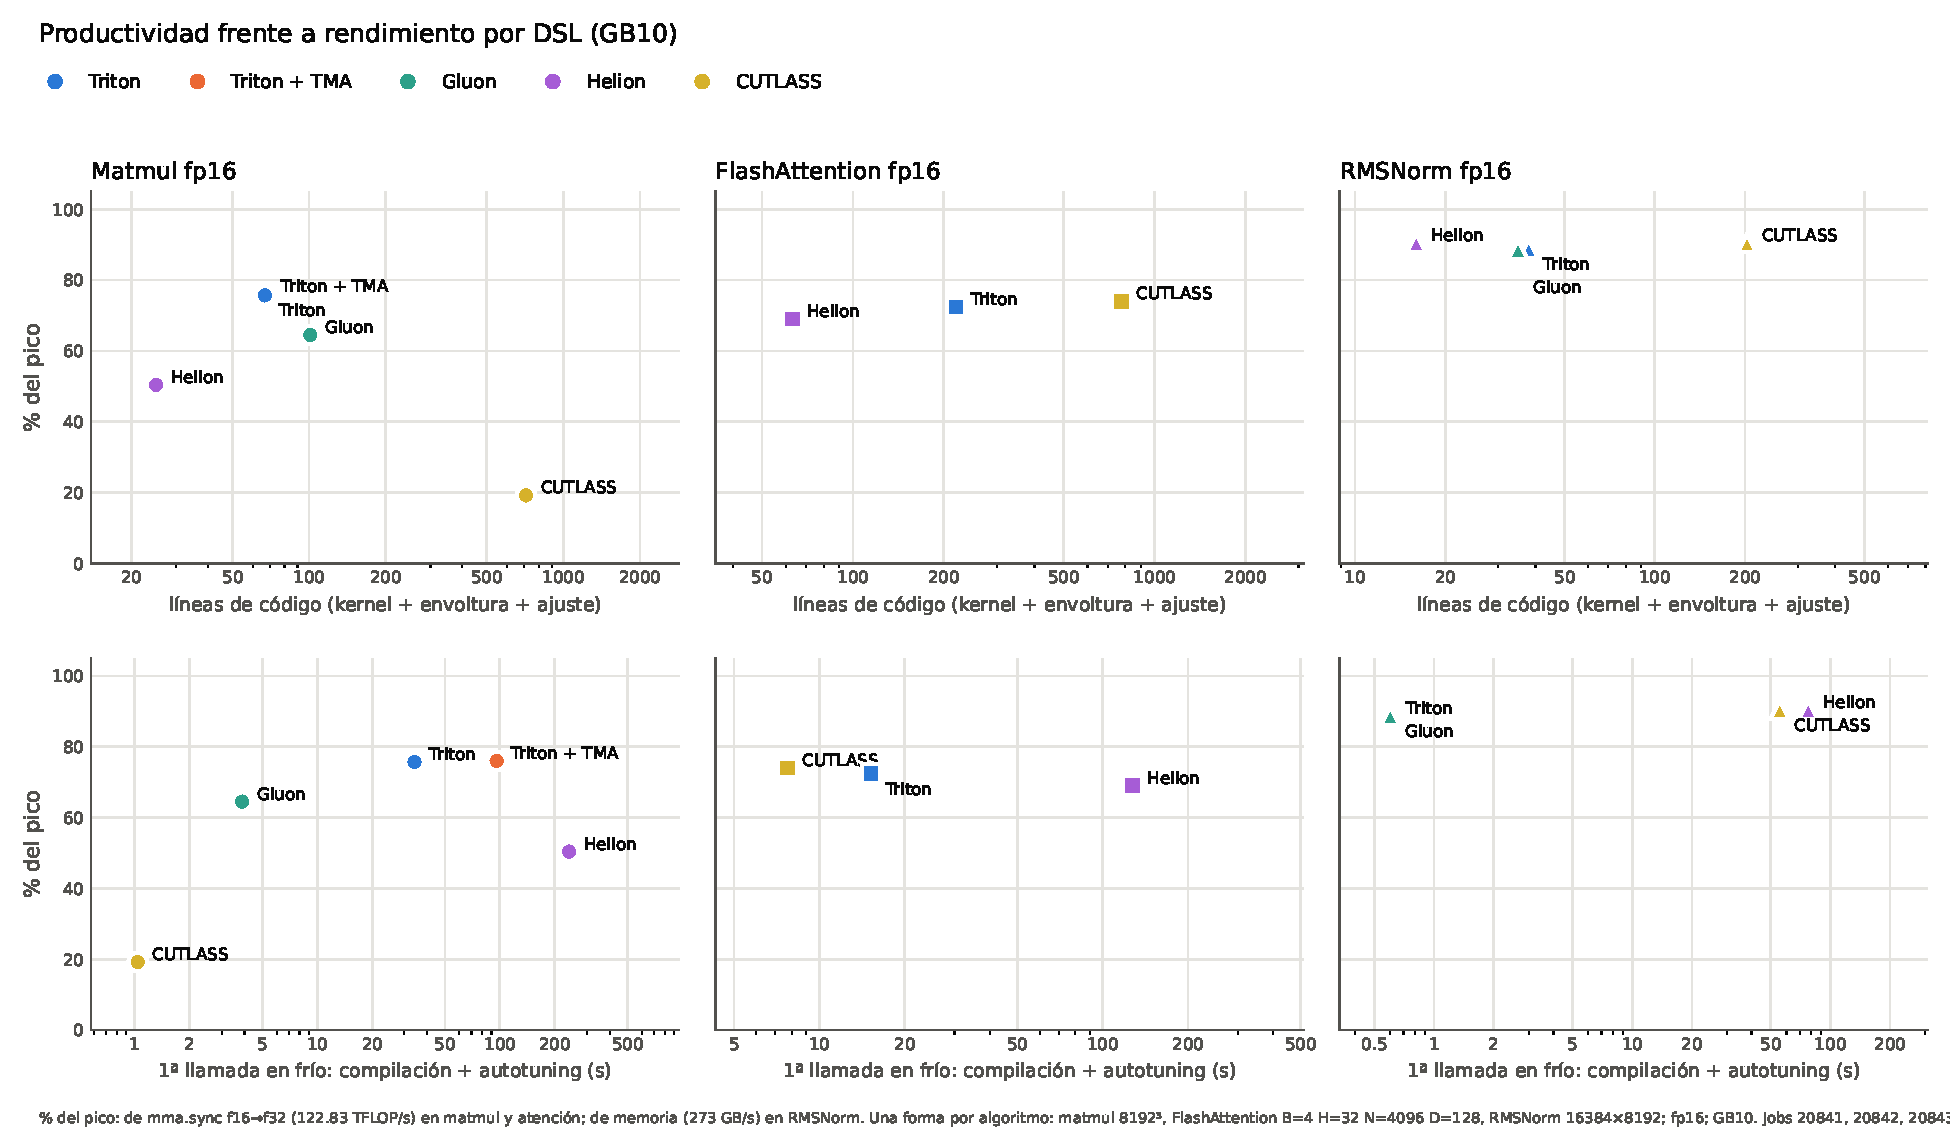
\includegraphics[width=\linewidth]{resultados/figuras/productividad.pdf}
  \caption{Rendimiento (\% del pico) frente a líneas de código (arriba) y frente al tiempo de
  la primera llamada en frío (abajo), por algoritmo. GB10, jobs 20841--20843.}
  \label{fig:productividad}
\end{figure}

\begin{table}[htbp]
  \centering\small
  \begin{tabular}{llrrlrrr}
    \toprule
    algoritmo & DSL & LoC total & LoC propias & ajuste & configs & 1ª llamada & \% pico \\
    \midrule
    Matmul & Triton & 67 & 67 & autotune & 64 & 34{,}1~s & 76 \\
    Matmul & Triton + TMA & 68 & 68 & autotune & 128 & 96{,}1~s & 76 \\
    Matmul & Gluon & 101 & 101 & barrido propio & 7 & 3{,}9~s & 65 \\
    Matmul & Helion & 25 & 25 & autotune (quick) & 251 & 4{,}0~min & 50 \\
    Matmul & CuTe & 713 & 41 & fija & 1 & 1{,}0~s & 19 \\
    \midrule
    FlashAttention & Triton & 220 & 220 & autotune & 36 & 15{,}2~s & 72 \\
    FlashAttention & Helion & 63 & 18 & autotune (quick) & 135 & 2{,}1~min & 69 \\
    FlashAttention & CuTe & 778 & 65 & barrido propio & 6 & 7{,}7~s & 74 \\
    \midrule
    RMSNorm & Triton & 38 & 38 & heurística & 1 & 0{,}6~s & 89 \\
    RMSNorm & Gluon & 35 & 35 & heurística & 1 & 0{,}6~s & 89 \\
    RMSNorm & Helion & 16 & 16 & autotune (quick) & 134 & 77{,}3~s & 90 \\
    RMSNorm & CUTLASS & 203 & 68 & fija & 1 & 55{,}5~s & 90 \\
    \bottomrule
  \end{tabular}
  \caption{Productividad frente a rendimiento en GB10. ``LoC propias'': las escritas en el TFM;
  el resto es código oficial reutilizado. RMSNorm de TLX (52 líneas) no compila en GB10. Los
  55{,}5~s de CUTLASS RMSNorm son la compilación con nvcc de la extensión.}
  \label{tab:productividad}
\end{table}

\subsection{Análisis}

\begin{enumerate}
  \item \textbf{Helion es el más conciso} (16--45 líneas por algoritmo, de 2 a 4 veces menos que
  Triton), pero lo paga en tiempo de ajuste: busca 134--251 configuraciones en 1{,}3--4~min por
  forma (hasta 31~min en atención con $N=16384$). Iguala al resto en RMSNorm, se queda cerca en
  atención y queda claramente por detrás en matmul (50\,\% frente a 76\,\%).
  \item \textbf{Triton es el punto de equilibrio}: 38--220 líneas, autotuning integrado de
  15--96~s y el mejor o casi el mejor rendimiento en los tres algoritmos.
  \item \textbf{CuTe exige un orden de magnitud más de código} (670--710 líneas el kernel
  oficial). A cambio es el más rápido en atención, con un ajuste barato (6 candidatas en
  7{,}7~s). Pero su ejemplo oficial de matmul para Blackwell GeForce rinde solo el 19\,\% en
  GB10, cuando en la RTX 5090 iguala a cuBLAS (99\,\% en el mismo job). No es por el número de
  clusters persistentes (sonda, job 20844), y barriendo el tile llega como mucho al 31\,\% (job
  20846): es un problema abierto de portabilidad entre sm\_120 y sm\_121.
  \item \textbf{Gluon cuesta más que Triton y rinde menos en matmul} (101 frente a 67 líneas;
  65 frente a 76\,\%): sin autotuner, el espacio que se explora a mano es pequeño. En RMSNorm
  equivale a Triton.
  \item \textbf{En un operador \emph{memory-bound} el DSL apenas importa para el rendimiento}
  (89--90\,\% en todos), pero sí para el coste: de 16 líneas y 77~s de autotuning a 203 líneas y
  55~s de nvcc.
  \item \textbf{El tiempo de ajuste es una dimensión propia}: va de 0{,}6~s a 4~min por forma
  con rendimientos parecidos, y en un uso con muchas formas se multiplica por su número.
\end{enumerate}

\subsection{Conclusión}

No hay un DSL dominante. Triton ofrece el mejor compromiso entre código, tiempo de ajuste y
rendimiento. Helion minimiza el código, pero traslada el esfuerzo al autotuning y en matmul no
alcanza a Triton. CUTLASS/CuTe maximiza el control a cambio de un orden de magnitud más de
código, y su matmul de ejemplo no es portable de sm\_120 a sm\_121 sin reajustarlo. Gluon solo
compensa cuando hace falta controlar el layout. Hay que tener en cuenta que las líneas de código
miden tamaño, no esfuerzo: una línea de CuTe no cuesta lo mismo que una de Helion.
. Requiere: \usepackage{graphicx,booktabs}.
% Datos: results/hennessy-frio (jobs 20841--20843, cache vacia) y benchmarks/productividad.py.

\section{Productividad frente a rendimiento de cada DSL}
\label{sec:productividad}

El resumen por arquitectura compara los DSLs solo por rendimiento, pero lo que los distingue es
el compromiso entre cuánto hay que escribir y ajustar y cuánto rinde lo escrito. Esta sección lo
mide con tres indicadores reproducibles: líneas de código, coste del ajuste y rendimiento como
porcentaje del pico del hardware.

\subsection{Método}

\textbf{Líneas de código lógicas} (sin blancos, comentarios ni docstrings), separadas en
\emph{kernel} (el código del algoritmo, con su lanzador y su espacio de configuraciones),
\emph{envoltura} (código propio para cargar un kernel externo) y \emph{ajuste} (código propio
para elegir la configuración cuando el DSL no trae autotuning). Si el repositorio carga un
ejemplo oficial de fuera (CUTLASS, la atención de Helion), se cuenta ese código en la versión
fijada del TFM, y solo la parte del algoritmo. Del FlashAttention de Triton solo se cuenta el
\emph{forward}.

\textbf{Coste del ajuste:} tiempo de la primera llamada (compilación + autotuning o barrido +
primera ejecución) con todas las cachés de compilación vacías (modo \texttt{TFM\_CACHE\_FRIA=1}
de \texttt{ejecutar.sh}). Antes de este modo la caché de Triton era persistente, y los tiempos
guardados mezclaban compilaciones en frío y en caliente. El tamaño del espacio de
configuraciones sale del código, o del log en el caso de Helion.

\textbf{Forma:} una por algoritmo, común a todos los DSLs, en fp16: matmul $8192^3$,
FlashAttention $B=4$, $H=32$, $N=4096$, $D=128$ sin máscara causal, y RMSNorm
$16384\times 8192$. El porcentaje del pico se calcula frente a \texttt{mma.sync} f16$\to$f32
(122{,}7~TFLOP/s, §~\ref{sec:pico-mma}) o frente al ancho de banda teórico (273~GB/s) en
RMSNorm.

\subsection{Resultados}

\begin{figure}[htbp]
  \centering
  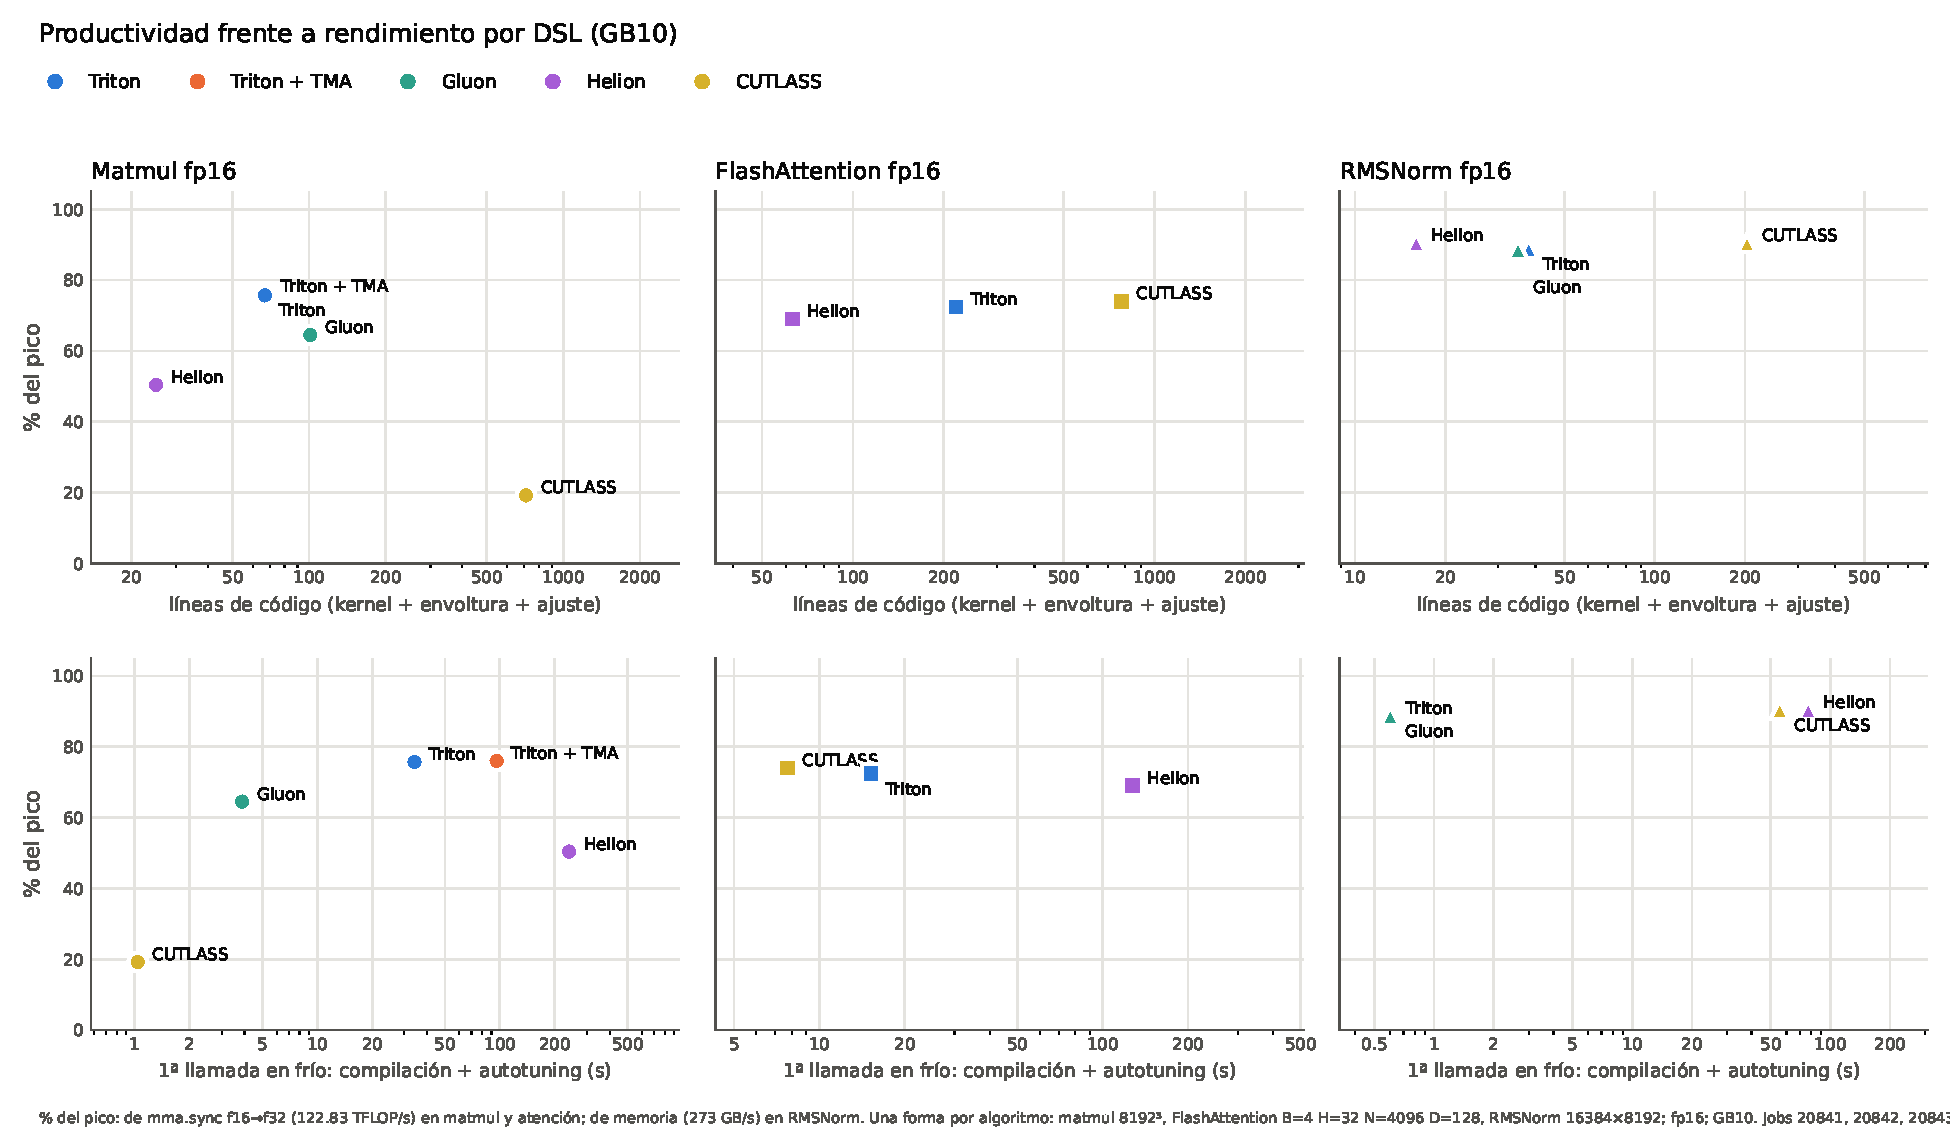
\includegraphics[width=\linewidth]{resultados/figuras/productividad.pdf}
  \caption{Rendimiento (\% del pico) frente a líneas de código (arriba) y frente al tiempo de
  la primera llamada en frío (abajo), por algoritmo. GB10, jobs 20841--20843.}
  \label{fig:productividad}
\end{figure}

\begin{table}[htbp]
  \centering\small
  \begin{tabular}{llrrlrrr}
    \toprule
    algoritmo & DSL & LoC total & LoC propias & ajuste & configs & 1ª llamada & \% pico \\
    \midrule
    Matmul & Triton & 67 & 67 & autotune & 64 & 34{,}1~s & 76 \\
    Matmul & Triton + TMA & 68 & 68 & autotune & 128 & 96{,}1~s & 76 \\
    Matmul & Gluon & 101 & 101 & barrido propio & 7 & 3{,}9~s & 65 \\
    Matmul & Helion & 25 & 25 & autotune (quick) & 251 & 4{,}0~min & 50 \\
    Matmul & CuTe & 713 & 41 & fija & 1 & 1{,}0~s & 19 \\
    \midrule
    FlashAttention & Triton & 220 & 220 & autotune & 36 & 15{,}2~s & 72 \\
    FlashAttention & Helion & 63 & 18 & autotune (quick) & 135 & 2{,}1~min & 69 \\
    FlashAttention & CuTe & 778 & 65 & barrido propio & 6 & 7{,}7~s & 74 \\
    \midrule
    RMSNorm & Triton & 38 & 38 & heurística & 1 & 0{,}6~s & 89 \\
    RMSNorm & Gluon & 35 & 35 & heurística & 1 & 0{,}6~s & 89 \\
    RMSNorm & Helion & 16 & 16 & autotune (quick) & 134 & 77{,}3~s & 90 \\
    RMSNorm & CUTLASS & 203 & 68 & fija & 1 & 55{,}5~s & 90 \\
    \bottomrule
  \end{tabular}
  \caption{Productividad frente a rendimiento en GB10. ``LoC propias'': las escritas en el TFM;
  el resto es código oficial reutilizado. RMSNorm de TLX (52 líneas) no compila en GB10. Los
  55{,}5~s de CUTLASS RMSNorm son la compilación con nvcc de la extensión.}
  \label{tab:productividad}
\end{table}

\subsection{Análisis}

\begin{enumerate}
  \item \textbf{Helion es el más conciso} (16--45 líneas por algoritmo, de 2 a 4 veces menos que
  Triton), pero lo paga en tiempo de ajuste: busca 134--251 configuraciones en 1{,}3--4~min por
  forma (hasta 31~min en atención con $N=16384$). Iguala al resto en RMSNorm, se queda cerca en
  atención y queda claramente por detrás en matmul (50\,\% frente a 76\,\%).
  \item \textbf{Triton es el punto de equilibrio}: 38--220 líneas, autotuning integrado de
  15--96~s y el mejor o casi el mejor rendimiento en los tres algoritmos.
  \item \textbf{CuTe exige un orden de magnitud más de código} (670--710 líneas el kernel
  oficial). A cambio es el más rápido en atención, con un ajuste barato (6 candidatas en
  7{,}7~s). Pero su ejemplo oficial de matmul para Blackwell GeForce rinde solo el 19\,\% en
  GB10, cuando en la RTX 5090 iguala a cuBLAS (99\,\% en el mismo job). No es por el número de
  clusters persistentes (sonda, job 20844), y barriendo el tile llega como mucho al 31\,\% (job
  20846): es un problema abierto de portabilidad entre sm\_120 y sm\_121.
  \item \textbf{Gluon cuesta más que Triton y rinde menos en matmul} (101 frente a 67 líneas;
  65 frente a 76\,\%): sin autotuner, el espacio que se explora a mano es pequeño. En RMSNorm
  equivale a Triton.
  \item \textbf{En un operador \emph{memory-bound} el DSL apenas importa para el rendimiento}
  (89--90\,\% en todos), pero sí para el coste: de 16 líneas y 77~s de autotuning a 203 líneas y
  55~s de nvcc.
  \item \textbf{El tiempo de ajuste es una dimensión propia}: va de 0{,}6~s a 4~min por forma
  con rendimientos parecidos, y en un uso con muchas formas se multiplica por su número.
\end{enumerate}

\subsection{Conclusión}

No hay un DSL dominante. Triton ofrece el mejor compromiso entre código, tiempo de ajuste y
rendimiento. Helion minimiza el código, pero traslada el esfuerzo al autotuning y en matmul no
alcanza a Triton. CUTLASS/CuTe maximiza el control a cambio de un orden de magnitud más de
código, y su matmul de ejemplo no es portable de sm\_120 a sm\_121 sin reajustarlo. Gluon solo
compensa cuando hace falta controlar el layout. Hay que tener en cuenta que las líneas de código
miden tamaño, no esfuerzo: una línea de CuTe no cuesta lo mismo que una de Helion.
. Requiere: \usepackage{graphicx,booktabs}.
% Datos: results/hennessy-frio (jobs 20841--20843, cache vacia) y benchmarks/productividad.py.

\section{Productividad frente a rendimiento de cada DSL}
\label{sec:productividad}

El resumen por arquitectura compara los DSLs solo por rendimiento, pero lo que los distingue es
el compromiso entre cuánto hay que escribir y ajustar y cuánto rinde lo escrito. Esta sección lo
mide con tres indicadores reproducibles: líneas de código, coste del ajuste y rendimiento como
porcentaje del pico del hardware.

\subsection{Método}

\textbf{Líneas de código lógicas} (sin blancos, comentarios ni docstrings), separadas en
\emph{kernel} (el código del algoritmo, con su lanzador y su espacio de configuraciones),
\emph{envoltura} (código propio para cargar un kernel externo) y \emph{ajuste} (código propio
para elegir la configuración cuando el DSL no trae autotuning). Si el repositorio carga un
ejemplo oficial de fuera (CUTLASS, la atención de Helion), se cuenta ese código en la versión
fijada del TFM, y solo la parte del algoritmo. Del FlashAttention de Triton solo se cuenta el
\emph{forward}.

\textbf{Coste del ajuste:} tiempo de la primera llamada (compilación + autotuning o barrido +
primera ejecución) con todas las cachés de compilación vacías (modo \texttt{TFM\_CACHE\_FRIA=1}
de \texttt{ejecutar.sh}). Antes de este modo la caché de Triton era persistente, y los tiempos
guardados mezclaban compilaciones en frío y en caliente. El tamaño del espacio de
configuraciones sale del código, o del log en el caso de Helion.

\textbf{Forma:} una por algoritmo, común a todos los DSLs, en fp16: matmul $8192^3$,
FlashAttention $B=4$, $H=32$, $N=4096$, $D=128$ sin máscara causal, y RMSNorm
$16384\times 8192$. El porcentaje del pico se calcula frente a \texttt{mma.sync} f16$\to$f32
(122{,}7~TFLOP/s, §~\ref{sec:pico-mma}) o frente al ancho de banda teórico (273~GB/s) en
RMSNorm.

\subsection{Resultados}

\begin{figure}[htbp]
  \centering
  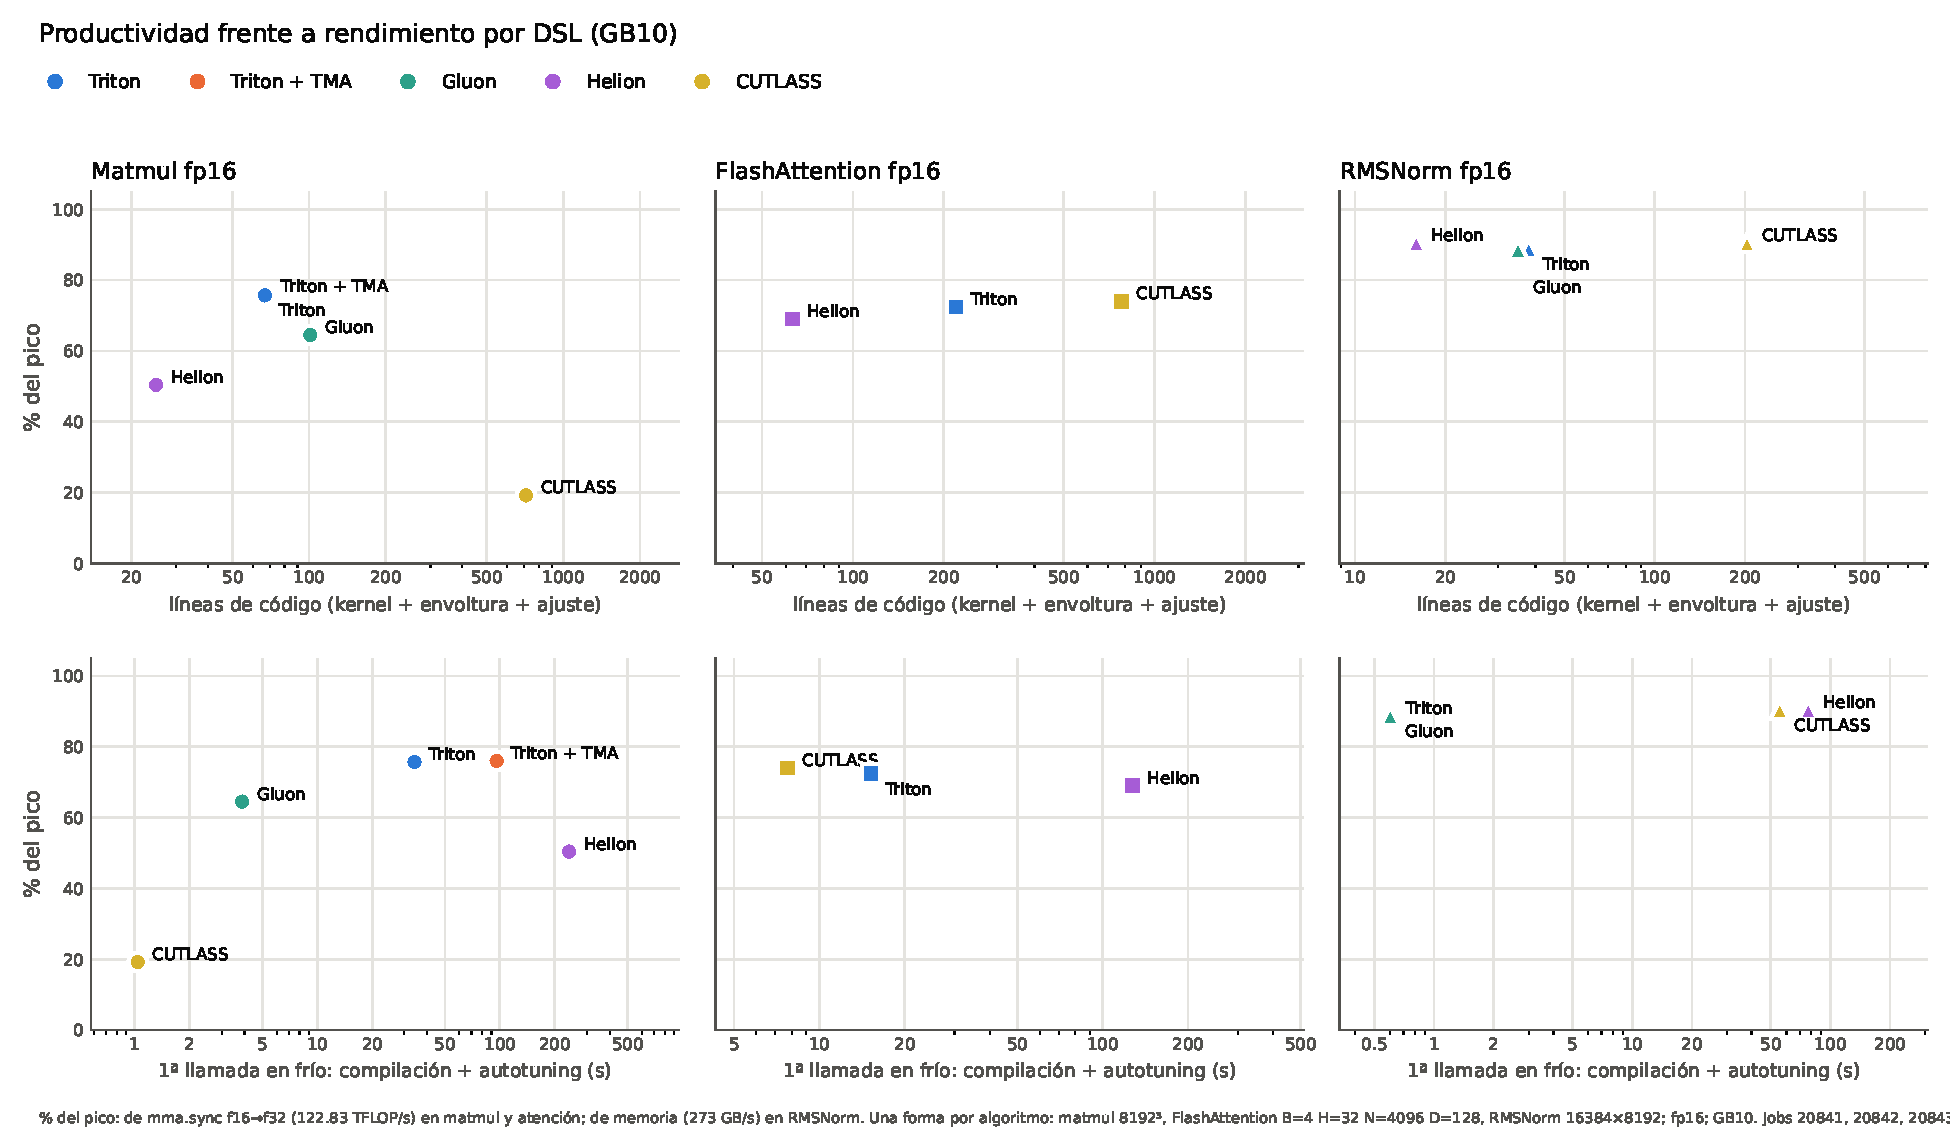
\includegraphics[width=\linewidth]{resultados/figuras/productividad.pdf}
  \caption{Rendimiento (\% del pico) frente a líneas de código (arriba) y frente al tiempo de
  la primera llamada en frío (abajo), por algoritmo. GB10, jobs 20841--20843.}
  \label{fig:productividad}
\end{figure}

\begin{table}[htbp]
  \centering\small
  \begin{tabular}{llrrlrrr}
    \toprule
    algoritmo & DSL & LoC total & LoC propias & ajuste & configs & 1ª llamada & \% pico \\
    \midrule
    Matmul & Triton & 67 & 67 & autotune & 64 & 34{,}1~s & 76 \\
    Matmul & Triton + TMA & 68 & 68 & autotune & 128 & 96{,}1~s & 76 \\
    Matmul & Gluon & 101 & 101 & barrido propio & 7 & 3{,}9~s & 65 \\
    Matmul & Helion & 25 & 25 & autotune (quick) & 251 & 4{,}0~min & 50 \\
    Matmul & CuTe & 713 & 41 & fija & 1 & 1{,}0~s & 19 \\
    \midrule
    FlashAttention & Triton & 220 & 220 & autotune & 36 & 15{,}2~s & 72 \\
    FlashAttention & Helion & 63 & 18 & autotune (quick) & 135 & 2{,}1~min & 69 \\
    FlashAttention & CuTe & 778 & 65 & barrido propio & 6 & 7{,}7~s & 74 \\
    \midrule
    RMSNorm & Triton & 38 & 38 & heurística & 1 & 0{,}6~s & 89 \\
    RMSNorm & Gluon & 35 & 35 & heurística & 1 & 0{,}6~s & 89 \\
    RMSNorm & Helion & 16 & 16 & autotune (quick) & 134 & 77{,}3~s & 90 \\
    RMSNorm & CUTLASS & 203 & 68 & fija & 1 & 55{,}5~s & 90 \\
    \bottomrule
  \end{tabular}
  \caption{Productividad frente a rendimiento en GB10. ``LoC propias'': las escritas en el TFM;
  el resto es código oficial reutilizado. RMSNorm de TLX (52 líneas) no compila en GB10. Los
  55{,}5~s de CUTLASS RMSNorm son la compilación con nvcc de la extensión.}
  \label{tab:productividad}
\end{table}

\subsection{Análisis}

\begin{enumerate}
  \item \textbf{Helion es el más conciso} (16--45 líneas por algoritmo, de 2 a 4 veces menos que
  Triton), pero lo paga en tiempo de ajuste: busca 134--251 configuraciones en 1{,}3--4~min por
  forma (hasta 31~min en atención con $N=16384$). Iguala al resto en RMSNorm, se queda cerca en
  atención y queda claramente por detrás en matmul (50\,\% frente a 76\,\%).
  \item \textbf{Triton es el punto de equilibrio}: 38--220 líneas, autotuning integrado de
  15--96~s y el mejor o casi el mejor rendimiento en los tres algoritmos.
  \item \textbf{CuTe exige un orden de magnitud más de código} (670--710 líneas el kernel
  oficial). A cambio es el más rápido en atención, con un ajuste barato (6 candidatas en
  7{,}7~s). Pero su ejemplo oficial de matmul para Blackwell GeForce rinde solo el 19\,\% en
  GB10, cuando en la RTX 5090 iguala a cuBLAS (99\,\% en el mismo job). No es por el número de
  clusters persistentes (sonda, job 20844), y barriendo el tile llega como mucho al 31\,\% (job
  20846): es un problema abierto de portabilidad entre sm\_120 y sm\_121.
  \item \textbf{Gluon cuesta más que Triton y rinde menos en matmul} (101 frente a 67 líneas;
  65 frente a 76\,\%): sin autotuner, el espacio que se explora a mano es pequeño. En RMSNorm
  equivale a Triton.
  \item \textbf{En un operador \emph{memory-bound} el DSL apenas importa para el rendimiento}
  (89--90\,\% en todos), pero sí para el coste: de 16 líneas y 77~s de autotuning a 203 líneas y
  55~s de nvcc.
  \item \textbf{El tiempo de ajuste es una dimensión propia}: va de 0{,}6~s a 4~min por forma
  con rendimientos parecidos, y en un uso con muchas formas se multiplica por su número.
\end{enumerate}

\subsection{Conclusión}

No hay un DSL dominante. Triton ofrece el mejor compromiso entre código, tiempo de ajuste y
rendimiento. Helion minimiza el código, pero traslada el esfuerzo al autotuning y en matmul no
alcanza a Triton. CUTLASS/CuTe maximiza el control a cambio de un orden de magnitud más de
código, y su matmul de ejemplo no es portable de sm\_120 a sm\_121 sin reajustarlo. Gluon solo
compensa cuando hace falta controlar el layout. Hay que tener en cuenta que las líneas de código
miden tamaño, no esfuerzo: una línea de CuTe no cuesta lo mismo que una de Helion.
. Requiere: \usepackage{graphicx,booktabs}.
% Datos: results/hennessy-frio (jobs 20841--20843, cache vacia) y benchmarks/productividad.py.

\section{Productividad frente a rendimiento de cada DSL}
\label{sec:productividad}

El resumen por arquitectura compara los DSLs solo por rendimiento, pero lo que los distingue es
el compromiso entre cuánto hay que escribir y ajustar y cuánto rinde lo escrito. Esta sección lo
mide con tres indicadores reproducibles: líneas de código, coste del ajuste y rendimiento como
porcentaje del pico del hardware.

\subsection{Método}

\textbf{Líneas de código lógicas} (sin blancos, comentarios ni docstrings), separadas en
\emph{kernel} (el código del algoritmo, con su lanzador y su espacio de configuraciones),
\emph{envoltura} (código propio para cargar un kernel externo) y \emph{ajuste} (código propio
para elegir la configuración cuando el DSL no trae autotuning). Si el repositorio carga un
ejemplo oficial de fuera (CUTLASS, la atención de Helion), se cuenta ese código en la versión
fijada del TFM, y solo la parte del algoritmo. Del FlashAttention de Triton solo se cuenta el
\emph{forward}.

\textbf{Coste del ajuste:} tiempo de la primera llamada (compilación + autotuning o barrido +
primera ejecución) con todas las cachés de compilación vacías (modo \texttt{TFM\_CACHE\_FRIA=1}
de \texttt{ejecutar.sh}). Antes de este modo la caché de Triton era persistente, y los tiempos
guardados mezclaban compilaciones en frío y en caliente. El tamaño del espacio de
configuraciones sale del código, o del log en el caso de Helion.

\textbf{Forma:} una por algoritmo, común a todos los DSLs, en fp16: matmul $8192^3$,
FlashAttention $B=4$, $H=32$, $N=4096$, $D=128$ sin máscara causal, y RMSNorm
$16384\times 8192$. El porcentaje del pico se calcula frente a \texttt{mma.sync} f16$\to$f32
(122{,}7~TFLOP/s, §~\ref{sec:pico-mma}) o frente al ancho de banda teórico (273~GB/s) en
RMSNorm.

\subsection{Resultados}

\begin{figure}[htbp]
  \centering
  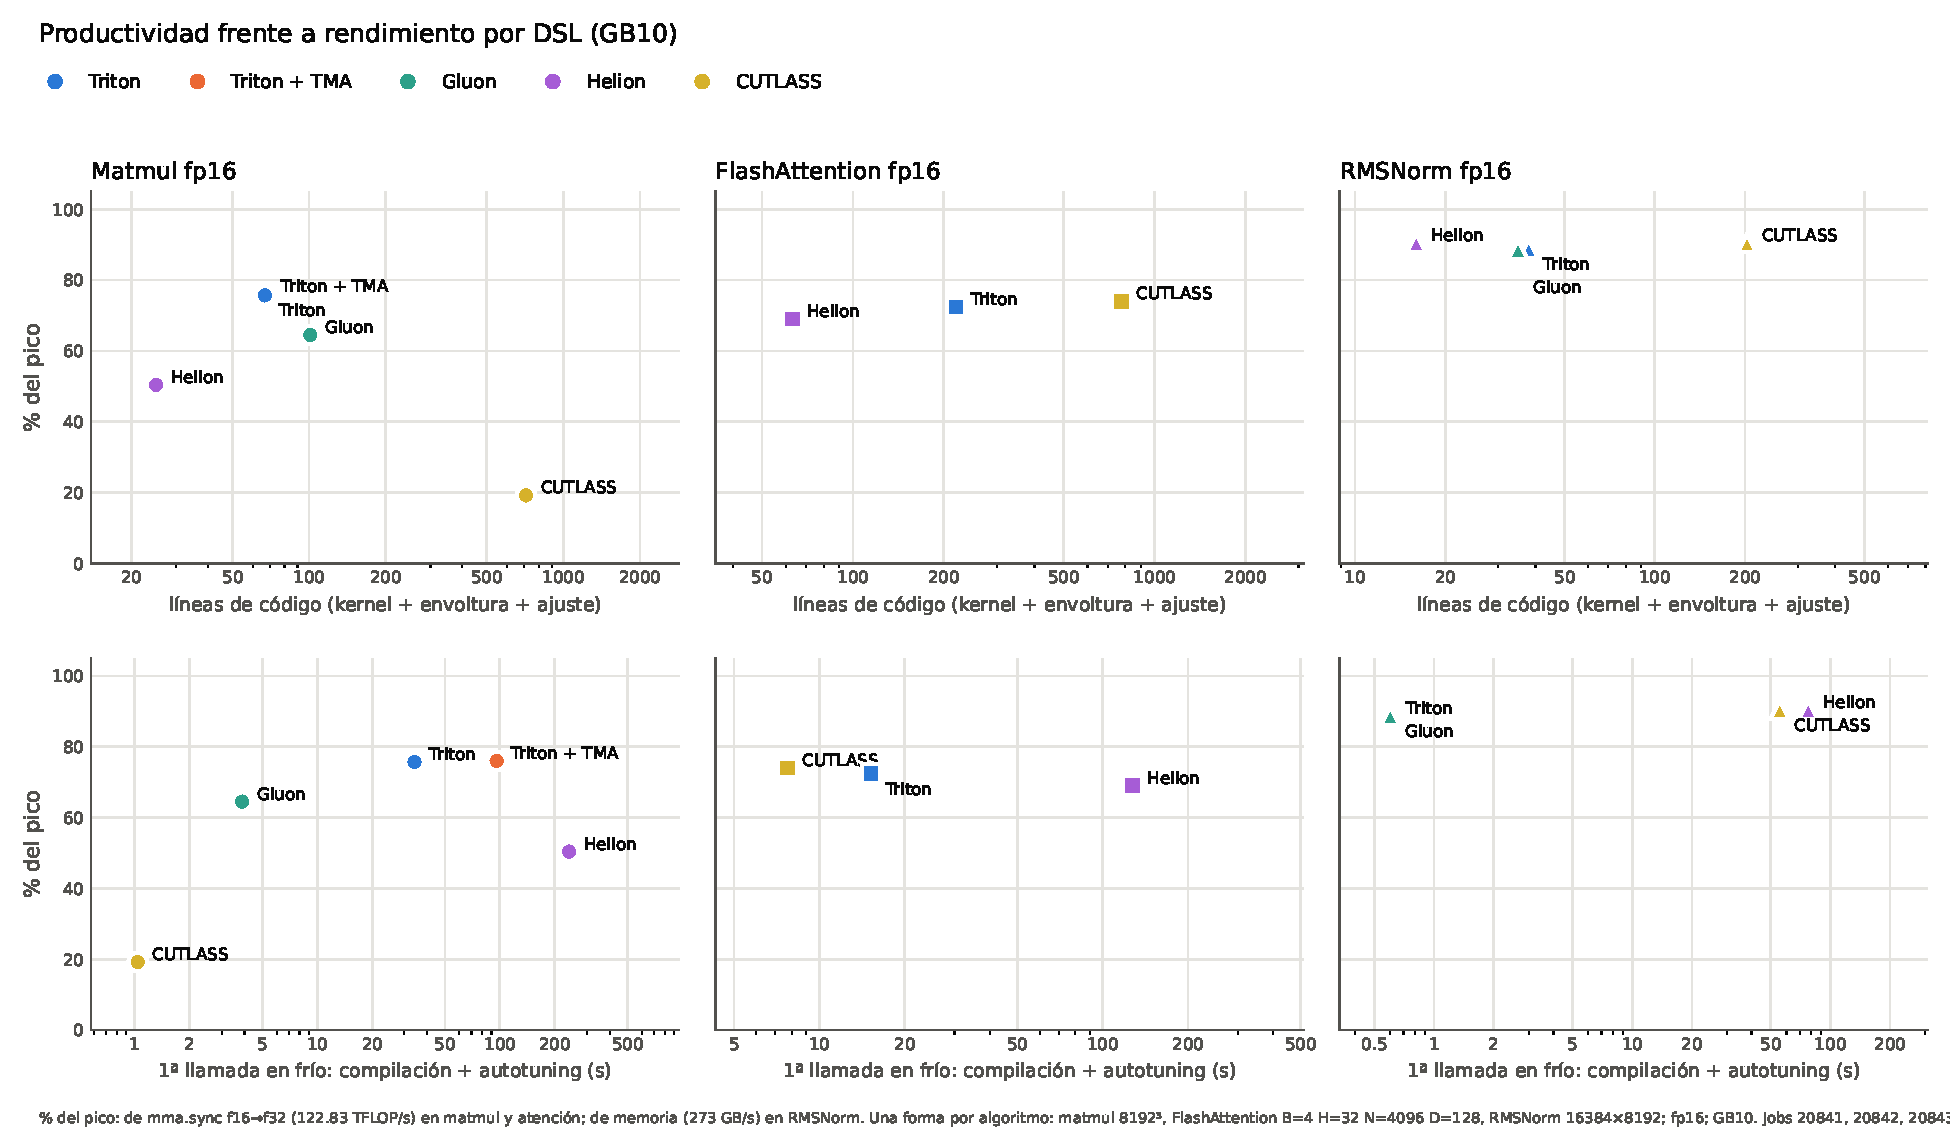
\includegraphics[width=\linewidth]{resultados/figuras/productividad.pdf}
  \caption{Rendimiento (\% del pico) frente a líneas de código (arriba) y frente al tiempo de
  la primera llamada en frío (abajo), por algoritmo. GB10, jobs 20841--20843.}
  \label{fig:productividad}
\end{figure}

\begin{table}[htbp]
  \centering\small
  \begin{tabular}{llrrlrrr}
    \toprule
    algoritmo & DSL & LoC total & LoC propias & ajuste & configs & 1ª llamada & \% pico \\
    \midrule
    Matmul & Triton & 67 & 67 & autotune & 64 & 34{,}1~s & 76 \\
    Matmul & Triton + TMA & 68 & 68 & autotune & 128 & 96{,}1~s & 76 \\
    Matmul & Gluon & 101 & 101 & barrido propio & 7 & 3{,}9~s & 65 \\
    Matmul & Helion & 25 & 25 & autotune (quick) & 251 & 4{,}0~min & 50 \\
    Matmul & CuTe & 713 & 41 & fija & 1 & 1{,}0~s & 19 \\
    \midrule
    FlashAttention & Triton & 220 & 220 & autotune & 36 & 15{,}2~s & 72 \\
    FlashAttention & Helion & 63 & 18 & autotune (quick) & 135 & 2{,}1~min & 69 \\
    FlashAttention & CuTe & 778 & 65 & barrido propio & 6 & 7{,}7~s & 74 \\
    \midrule
    RMSNorm & Triton & 38 & 38 & heurística & 1 & 0{,}6~s & 89 \\
    RMSNorm & Gluon & 35 & 35 & heurística & 1 & 0{,}6~s & 89 \\
    RMSNorm & Helion & 16 & 16 & autotune (quick) & 134 & 77{,}3~s & 90 \\
    RMSNorm & CUTLASS & 203 & 68 & fija & 1 & 55{,}5~s & 90 \\
    \bottomrule
  \end{tabular}
  \caption{Productividad frente a rendimiento en GB10. ``LoC propias'': las escritas en el TFM;
  el resto es código oficial reutilizado. RMSNorm de TLX (52 líneas) no compila en GB10. Los
  55{,}5~s de CUTLASS RMSNorm son la compilación con nvcc de la extensión.}
  \label{tab:productividad}
\end{table}

\subsection{Análisis}

\begin{enumerate}
  \item \textbf{Helion es el más conciso} (16--45 líneas por algoritmo, de 2 a 4 veces menos que
  Triton), pero lo paga en tiempo de ajuste: busca 134--251 configuraciones en 1{,}3--4~min por
  forma (hasta 31~min en atención con $N=16384$). Iguala al resto en RMSNorm, se queda cerca en
  atención y queda claramente por detrás en matmul (50\,\% frente a 76\,\%).
  \item \textbf{Triton es el punto de equilibrio}: 38--220 líneas, autotuning integrado de
  15--96~s y el mejor o casi el mejor rendimiento en los tres algoritmos.
  \item \textbf{CuTe exige un orden de magnitud más de código} (670--710 líneas el kernel
  oficial). A cambio es el más rápido en atención, con un ajuste barato (6 candidatas en
  7{,}7~s). Pero su ejemplo oficial de matmul para Blackwell GeForce rinde solo el 19\,\% en
  GB10, cuando en la RTX 5090 iguala a cuBLAS (99\,\% en el mismo job). No es por el número de
  clusters persistentes (sonda, job 20844), y barriendo el tile llega como mucho al 31\,\% (job
  20846): es un problema abierto de portabilidad entre sm\_120 y sm\_121.
  \item \textbf{Gluon cuesta más que Triton y rinde menos en matmul} (101 frente a 67 líneas;
  65 frente a 76\,\%): sin autotuner, el espacio que se explora a mano es pequeño. En RMSNorm
  equivale a Triton.
  \item \textbf{En un operador \emph{memory-bound} el DSL apenas importa para el rendimiento}
  (89--90\,\% en todos), pero sí para el coste: de 16 líneas y 77~s de autotuning a 203 líneas y
  55~s de nvcc.
  \item \textbf{El tiempo de ajuste es una dimensión propia}: va de 0{,}6~s a 4~min por forma
  con rendimientos parecidos, y en un uso con muchas formas se multiplica por su número.
\end{enumerate}

\subsection{Conclusión}

No hay un DSL dominante. Triton ofrece el mejor compromiso entre código, tiempo de ajuste y
rendimiento. Helion minimiza el código, pero traslada el esfuerzo al autotuning y en matmul no
alcanza a Triton. CUTLASS/CuTe maximiza el control a cambio de un orden de magnitud más de
código, y su matmul de ejemplo no es portable de sm\_120 a sm\_121 sin reajustarlo. Gluon solo
compensa cuando hace falta controlar el layout. Hay que tener en cuenta que las líneas de código
miden tamaño, no esfuerzo: una línea de CuTe no cuesta lo mismo que una de Helion.
